\documentclass{beamer}
\usetheme{metropolis}
\usepackage{graphicx}
\usepackage{amsmath}
\usepackage{tcolorbox}
\title{Digital Signal Processing: COSC390}
\author{Jordan Hanson}
\institute{Whittier College Department of Physics and Astronomy}

\begin{document}
\maketitle

\begin{frame}{Unit 1.3 Outline}
Previous lectures covered:
\begin{itemize}
\item Complex numbers 2: The Fourier series and Fourier transform (continuous and discrete)
\item \textit{Time-permitting}: The Laplace transform (continuous and discrete)
\end{itemize}
This lecture will cover: (Reading: \textbf{Chapter 2})
\begin{itemize}
\item \alert{Statistics and probability: the normal distribution and other useful distributions}
\item \alert{Noise: digitization and sampling}
\item Noise: Spectral properties of noise, ADC and DAC
\end{itemize}
\end{frame}

\section{Statistics and Probability: The Normal Distribution}

\begin{frame}[fragile]{Statistics and Probability: The Normal Distribution}
The \textit{mean}, $\mu$, and \textit{standard deviation}, $\sigma$, of a data set $\lbrace x_i \rbrace$ are defined as
\begin{align}
\mu &= \frac{1}{N}\sum_{i=1}^N x_i \\
\sigma^2 &= \frac{1}{N-1}\sum_{i=1}^N\left(x_i-\mu\right)^2
\end{align}
Octave commands:
\begin{verbatim}
x = randn(100,1);
mean(x)
std(x)
\end{verbatim}
\end{frame}

\begin{frame}[fragile]{Statistics and Probability: The Normal Distribution}
One nice theorem: \textit{The variance is the average of the squares minus the square of the average.}  Let $\langle x \rangle$ represent the average of the quantity or expression $x$.  We have
\begin{equation}
\sigma_x^2 = \langle x^2 \rangle - \langle x \rangle^2
\end{equation}
Proof: observe on board.
\end{frame}

\begin{frame}[fragile]{Statistics and Probability: The Normal Distribution}
\small
\textbf{Note}: There is a distinction between the \textit{process or signal process} and the \textit{the data}.  Just because the data has a given $\mu$ and $\sigma$ does not imply that the signal process has or will continue to have the exact same values of $\mu$ and $\sigma$.  The underlying process could be \textit{non-stationary}.
\begin{figure}
\centering
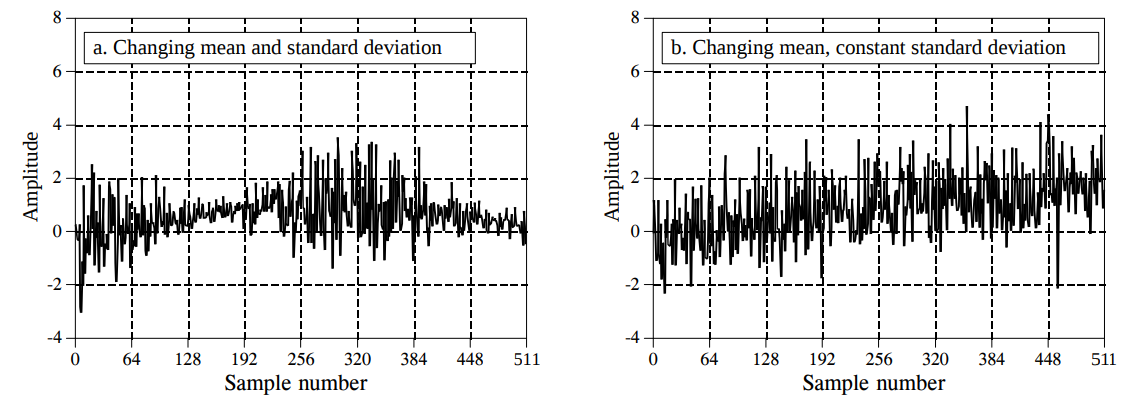
\includegraphics[width=0.9\textwidth]{figures/non_stationary.png}
\caption{\label{fig:non_stationary} Signal processes in (a) and (b) are considered \alert{non-stationary} because one or both of $\mu$ and $\sigma$ depend on time.}
\end{figure}
\end{frame}

\begin{frame}[fragile]{Statistics and Probability: The Normal Distribution}
\small
\textbf{A histogram} is an object that represents the frequency\footnote{Careful: the word frequency refers to the number of occurences in the data, not a sinusoidal frequency.} of particular values in a signal.  For example, below is a histogram of 256,000 numbers drawn from a probability distribution:
\begin{figure}
\centering
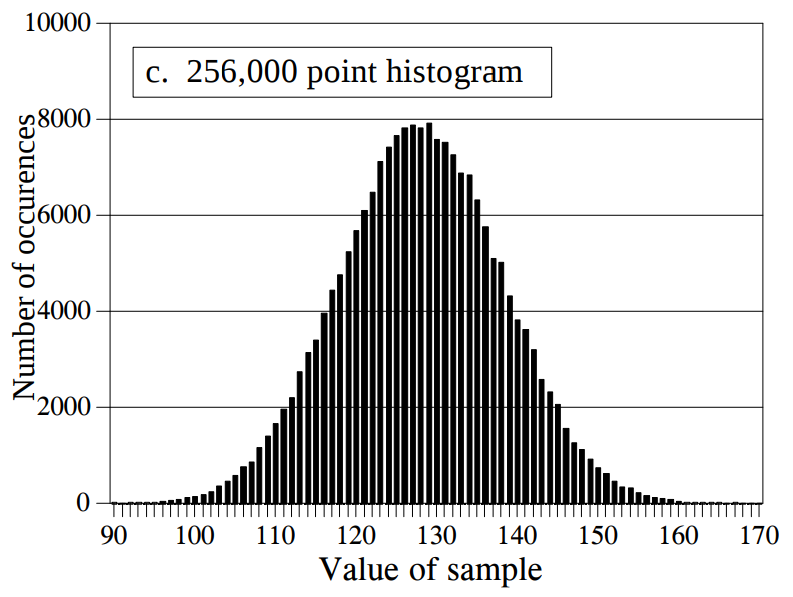
\includegraphics[width=0.45\textwidth]{figures/hist.png}
\caption{\label{fig:hist} The histogram contains counts versus sample values.}
\end{figure}
\end{frame}

\begin{frame}[fragile]{Statistics and Probability: The Normal Distribution}
The following octave code should reproduce something like Fig. \ref{fig:hist} from the textbook:
\begin{verbatim}
x = randn(256000,1)*10.0+130.0;
[b,a] = hist(x,100);
plot(a,b,'o');
\end{verbatim}
The function \textit{randn(N,M)} draws $N \times M$ numbers from a normal distribution and returns them in the size the user desires.  The function \textit{hist(x,N)} creates $N$ bins and sorts the data $x_i$ into them.
\end{frame}

\begin{frame}[fragile]{Statistics and Probability: The Normal Distribution}
\small
For data that is appropriately stationary, we can use histograms to estimate $\mu$ and $\sigma$ faster, since we only have to loop over bins rather than every data sample.  Let $H_i$ represent the counts in a given bin, and $i$ represent the bin sample.  We have:
\begin{align}
\mu &= \frac{1}{N}\sum_{i=1}^{M}i H_i \\
\sigma^{2} &= \frac{1}{N-1}\sum_{i=1}^M \left(i-\mu\right)^2 H_i
\end{align}
(To obtain the mean in signal \textit{amplitude}, you'd have to convert bin number to amplitude - more on that in a moment).
\end{frame}

\begin{frame}[fragile]{Statistics and Probability: The Normal Distribution}
\small
Some vocabulary:
\begin{itemize}
\item \textbf{normalization} - Total probability is 1.0.  For pdf - the integral from $[-\infty,\infty]$ is 1.0.  For pmf - the sum from $[-\infty,\infty]$ is 1.0.
\item \textbf{pmf} - Probability mass function: A \textit{normalized continuous function} that gives the probability of a value, given the value.
\item \textbf{histogram} - Histograms are an attempted measurement of the pmf by breaking the data into discrete bins.  Histograms can be \textit{normalized} as well.
\item \textbf{pdf} - Probability density function: A \textit{normalized continuous function} that gives the probability density of a value, given the value.  Integrating the \textit{normalized} pdf between two values gives the probability of observing data between the given values.
\end{itemize}
\end{frame}

\begin{frame}[fragile]{Statistics and Probability: The Normal Distribution}
\begin{figure}
\centering
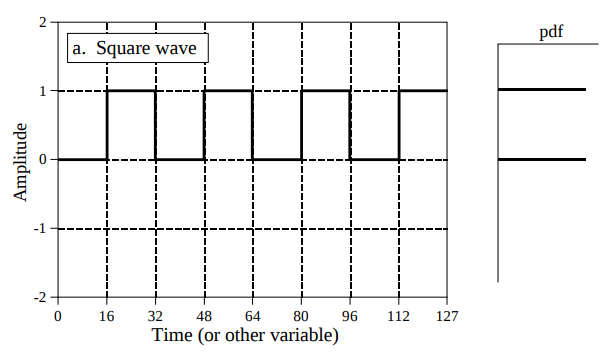
\includegraphics[width=0.7\textwidth]{figures/squarepdf.png}
\caption{\label{fig:squarepdf} The square-wave signal spends equal time at 0.0 and 1.0, and the probability density function reflects that.}
\end{figure}
\end{frame}

\begin{frame}[fragile]{Statistics and Probability: The Normal Distribution}
\begin{figure}
\centering
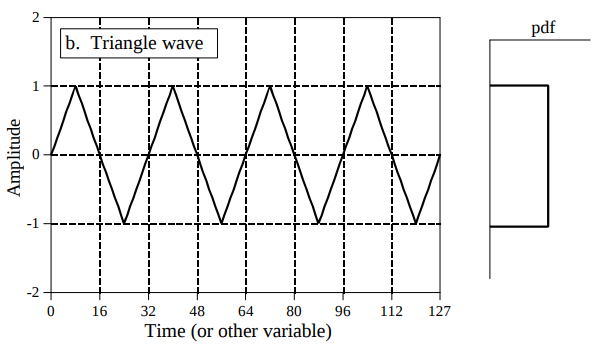
\includegraphics[width=0.7\textwidth]{figures/trianglepdf.png}
\caption{\label{fig:trianglepdf} The triangle-wave signal spends equal time at all values \textit{between} 0.0 and 1.0, and the probability density function reflects that.}
\end{figure}
\end{frame}

\begin{frame}[fragile]{Statistics and Probability: The Normal Distribution}
\begin{figure}
\centering
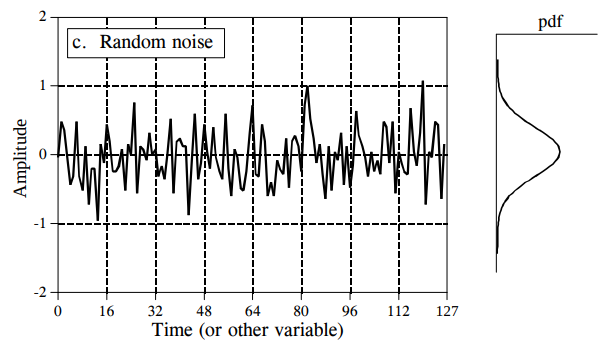
\includegraphics[width=0.7\textwidth]{figures/randnpdf.png}
\caption{\label{fig:randnpdf} The random noise \textit{usually} spends time near 0.0, but rarely it fluctuates to larger values.}
\end{figure}
\end{frame}

\begin{frame}{Normal distribution}
\textbf{Normally distributed} data decreases in probability at a rate that is proportional (1) to the \textit{distance from the mean}, and that is proportional (2) to the \textit{probability itself.}
\begin{figure}
\centering
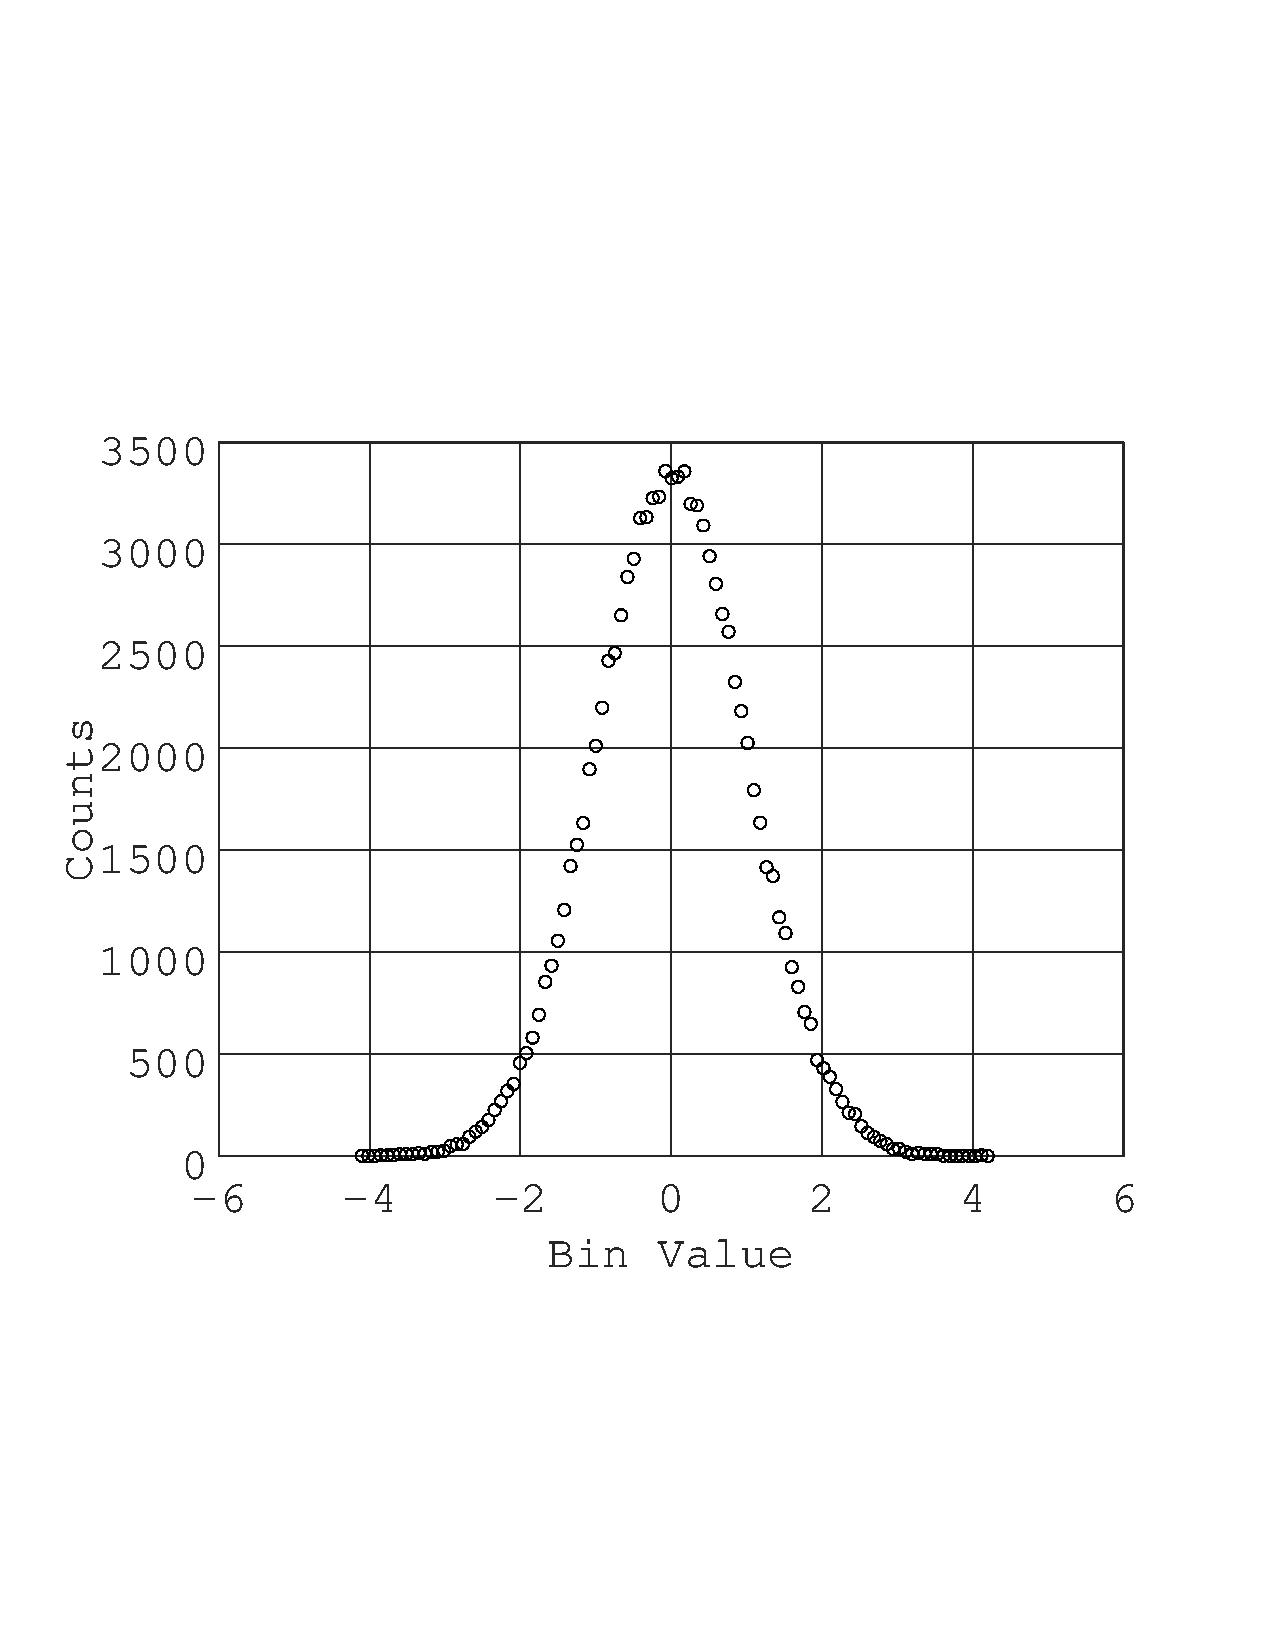
\includegraphics[width=0.5\textwidth,trim=0cm 6cm 0cm 6cm,clip=true]{figures/hist_binCount.pdf}
\caption{\label{fig:hist1} Normally distributed data counts decrease as measured further from the mean for \textit{two reasons.}}
\end{figure}
\end{frame}

\begin{frame}{Normal distribution}
\begin{tcolorbox}[colback=white,colframe=red!40!blue,title=Normal Distribution PDF]
\alert{Let $p(x)$ be the PDF of normally distributed data $x$ with mean $\mu$. In order to obey conditions (1) and (2), the function $p(x)$ must be described by the following differential equation, where $k$ is some constant.}
\alert{\begin{equation}
\frac{dp}{dx} = -k(x-\mu)p(x) \label{eq:normDiffeq}
\end{equation}}
\end{tcolorbox}
\end{frame}

\begin{frame}{Normal distribution}
Rearranging Eq. \ref{eq:normDiffeq}, we have
\begin{equation}
\frac{dp}{p} = -k(x-\mu) dx
\end{equation}
Integrating both sides gives
\begin{equation}
\ln(p) = -\frac{1}{2}k(x-\mu)^2+C_0
\end{equation}
Exponentiating,
\begin{equation}
p(x) = C_1 \exp\left(-\frac{1}{2}k(x-\mu)^2\right) \label{eq:normDiffeq2}
\end{equation}
Ensuring that the PDF is \textit{normalized} requires
\begin{equation}
\int_{-\infty}^{\infty} p(x) dx = 1
\end{equation}
\end{frame}

\begin{frame}{Normal distribution}
But how do we integrate Eq. \ref{eq:normDiffeq2}?  First, a change of variables.  Let $s = \sqrt{k/2}(x-\mu)$, so $ds = \sqrt{k/2}dx$.  Then, we have
\begin{equation}
C_1 \sqrt{\frac{2}{k}} \int_{-\infty}^{\infty} \exp(-s^2) ds = 1
\end{equation}
Squaring both sides, we have
\begin{equation}
C_1^2 \frac{2}{k} \left(\int_{-\infty}^{\infty} \exp(-s^2) ds\right)^2 = 1
\end{equation}
\end{frame}

\begin{frame}{Normal distribution}
Let's pretend the two factors of the integral involve different variables:
\begin{equation}
C_1^2 \frac{2}{k} \left(\int_{-\infty}^{\infty} \exp(-x^2) dx\right)\left(\int_{-\infty}^{\infty} \exp(-y^2) dy\right) = 1
\end{equation}
Now we have
\begin{equation}
C_1^2 \frac{2}{k} \int_{-\infty}^{\infty} \exp(-(x^2+y^2)) dx dy = 1
\end{equation}
Change to polar coordinates ($x^2 + y^2 = r^2$)
\begin{equation}
C_1^2 \frac{2}{k} \int_{0}^{\infty} \int_0^{2\pi} r\exp(-r^2) dr d\phi = 1
\end{equation}
\end{frame}

\begin{frame}{Normal distribution}
One more substitution: $u = r^2$, and $du = 2rdr$:
\begin{equation}
-\frac{C_1^2}{k} \int_0^{\infty}\int_0^{2\pi} \exp(-u) du d\phi = 1
\end{equation}
Solving for $C_1$, we find
\begin{equation}
C_1 = \sqrt{\frac{k}{2\pi}}
\end{equation}
Thus the pdf of normally distributed data is
\begin{equation}
p(x) = \sqrt{\frac{k}{2\pi}} \exp\left(-\frac{1}{2}k(x-\mu)^2\right)
\end{equation}
Let's defined $k = \frac{1}{\sigma_x^2}$ so that it's clear the exponent has the proper ratio of units:
\begin{equation}
\boxed{
p(x) = \sqrt{\frac{1}{2\pi\sigma_x^2}} \exp\left(-\frac{1}{2}\left(\frac{x-\mu}{\sigma_s}\right)^2\right)}
\end{equation}
\end{frame}

\section{Statistics and Probability: Programming with Octave}

\begin{frame}[fragile]{Statistics and Probability: Programming with Octave}
More on the \textit{hist} function in octave:
\begin{verbatim}
pkg install -forge io
pkg install -forge statistics
pkg load statistics
pkg help histfit
histfit(randn(1000,1))
histfit(rand(1000,1))
\end{verbatim}
Let's work out the $\sigma$ of a \textit{flat} distribution between $[0,1]$.  What is it for a flat distribution between $[-1,1]$?
\end{frame}

\section{Statistics and Probability: Other Useful Distributions}

\section{Conclusion}

\begin{frame}{Unit 1.3 Outline}
Previous lectures covered:
\begin{itemize}
\item Complex numbers 2: The Fourier series and Fourier transform (continuous and discrete)
\item \textit{Time-permitting}: The Laplace transform (continuous and discrete)
\end{itemize}
This lecture will cover: (Reading: \textbf{Chapter 2})
\begin{itemize}
\item \alert{Statistics and probability: the normal distribution and other useful distributions}
\item \alert{Noise: digitization and sampling}
\item Noise: Spectral properties of noise, ADC and DAC
\end{itemize}
\end{frame}

\end{document}
